\section{Method}
\label{sec:method}

We instantiate the decomposition from \S\ref{sec:decomp} in two spaces:
the residual stream, where it defines a block-level observable, and the
attention value space, where it isolates an attention-side source of parallel
updates. These two views lead to the component-scaling interventions used in
the experiments.

\begin{figure*}[t]
  \centering
  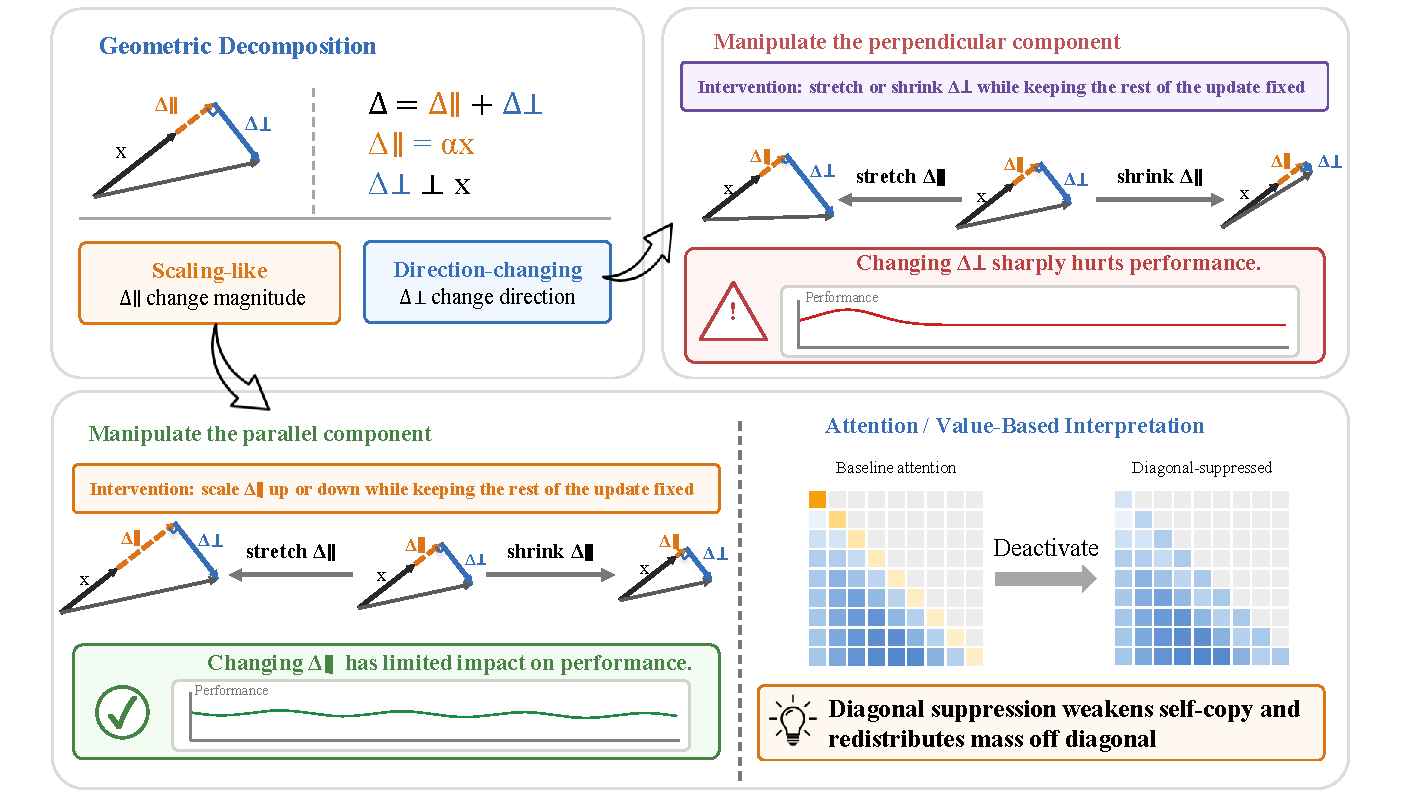
\includegraphics[width=0.98\textwidth]{figs/overview/parallel_updates_main_figure_analysis_v11_midline_arrows.pdf}
  \caption{\textbf{Overview of the method and its downstream use.}
           We first measure residual-update geometry at the block level, then
           trace the attention-side parallel component to the product of
           self-routing and value self-alignment. This factorization yields a
           unified component-scaling form for value- and residual-space edits,
           which we use in the experiments on inference-time editing,
           compression error, and pretraining behavior.}
  \label{fig:overview}
\end{figure*}

% ------------------------------------------------------------------
\subsection{Residual-Level Decomposition}
\label{sec:residual-level}

\paragraph{Instantiation.}
Set $\Delta = \Du{l}{t}$ (the residual update of block $f^l$ at token $t$)
and $\mathbf{z} = \hz{l}{t}$ (the pre-update hidden state).
For reporting layer and module profiles, we average the per-token residual
parallel ratio over a calibration corpus:
\begin{equation}
  \pr{l}{t}
  = r\!\left(\Du{l}{t},\,\hz{l}{t}\right)
  = \frac{|\alpha^l_t|\,\|\hz{l}{t}\|}{\|\Du{l}{t}\|},
  \quad
  \alpha^l_t
  = \frac{\Du{l}{t}\!\cdot\!\hz{l}{t}}{\|\hz{l}{t}\|^2},
  \quad
  \PR{l}
  = \mathbb{E}_{x,t}\!\left[\pr{l}{t}(x)\right].
  \label{eq:para-ratio}
\end{equation}
This residual-level view serves as the shared observable for the rest of the
paper. The resulting diagnostic is block-agnostic. We apply it to
(i)~the $\Attn$ sub-layer output,
(ii)~the $\FFN$ sub-layer output, and
(iii)~the combined block update.

% ------------------------------------------------------------------
\subsection{Value-Space Decomposition}
\label{sec:value-level}

\paragraph{Instantiation.}
Inside the attention computation, each token's own hidden state passes
through the value projection to become $\mathbf{v}_t = V\hz{}{t}$.
Set $\Delta = \mathbf{v}_t$ and $\mathbf{z} = \hz{}{t}$ (layer index
suppressed).  The parallel component of $\mathbf{v}_t$ with respect to
$\hz{}{t}$ is characterized by the scalar
\begin{equation}
  \varphi_t
    = \frac{\mathbf{v}_t\cdot\hz{}{t}}{\|\hz{}{t}\|^2},
  \label{eq:phi}
\end{equation}
which we call the \emph{value self-alignment}.
$\varphi_t > 0$ means the value projection partially preserves the direction
of the residual stream for a token's own representation; $\varphi_t = 0$
means it is purely perpendicular; $\varphi_t = 1$ means the parallel component
of $\mathbf{v}_t$ matches $\hz{}{t}$ in the same direction; and
$\varphi_t = -1$ means it matches the same scale in the opposite direction.

Residual-level geometry alone cannot identify which part of the attention
computation creates the parallel component. Moving the decomposition into
value space isolates the token's own contribution before attention
aggregation, which makes it possible to connect residual-stream geometry to
an explicit attention-side mechanism.

We apply this value-space analysis specifically to attention. The feed-forward
block also produces residual-level parallel and perpendicular components, but
its intermediate activation has a different channel dimension and lacks a
token-wise diagonal self-routing term. We therefore treat MLP outputs at the
residual level, while using value-space decomposition for the attention-side
source of parallel updates.

\paragraph{Attention-side factorization.}
Writing
$\mathbf{o}_t=\Adiag{t}\mathbf{v}_t+\sum_{s\neq t}\Aij{t}{s}\mathbf{v}_s$
for the value-space attention aggregation and projecting it onto $\hz{}{t}$
yields
\begin{equation}
  \alpha_t^{\Attn}
    = \underbrace{\Adiag{t}\cdot\varphi_t}_{\text{routing} \times \text{alignment}}
      \;+\; \underbrace{\sum_{s \neq t}\Aij{t}{s}\,
            \frac{\mathbf{v}_s\cdot\hz{}{t}}{\|\hz{}{t}\|^2}}_{\text{cross-token}}.
  \label{eq:alpha-attn}
\end{equation}
This factorization separates the diagonal self-value route from cross-token
aggregation. The diagonal term carries the token's own value vector, and its
projection onto the residual stream is exactly weighted by
$\Adiag{t}\varphi_t$. Thus changing the diagonal coefficient directly changes
the self-value-parallel contribution, whereas the cross-token term aggregates
non-self values and is not determined by the token's own diagonal route.

% ------------------------------------------------------------------
\subsection{Unified Component-Scaling Form}
\label{sec:closed-form-control}

Equation~\ref{eq:alpha-attn} links the diagonal attention coefficient to the
self-value-parallel contribution. To express interventions that either
suppress or amplify this contribution, we use a general
parallel-perpendicular rescaling form. Let
\begin{equation}
  \mathbf{y}_t = \sum_{s\le t} A_{ts}\mathbf{m}_s,\qquad
  \mathbf{y}_{t,\parallel}
    = \frac{\mathbf{y}_t^\top\mathbf{r}_t}{\|\mathbf{r}_t\|^2}\mathbf{r}_t,
  \qquad
  \mathbf{y}_{t,\perp}=\mathbf{y}_t-\mathbf{y}_{t,\parallel},
  \label{eq:unified-component-decomp}
\end{equation}
where $\mathbf{m}_s$ is the message vector being aggregated and
$\mathbf{r}_t$ is the reference direction used to define parallelness. The edited
output is
\begin{equation}
  \widetilde{\mathbf{y}}_t(s_{\parallel},s_{\perp})
    = s_{\parallel}\mathbf{y}_{t,\parallel}
      + s_{\perp}\mathbf{y}_{t,\perp}.
  \label{eq:unified-component-scaling}
\end{equation}
Here \(s_{\parallel}\) and \(s_{\perp}\) are multiplicative scales applied to
the parallel and perpendicular components, respectively. The unedited baseline
is \(s_{\parallel}=s_{\perp}=1\). Parallel removal sets
\(s_{\parallel}=0,s_{\perp}=1\), perpendicular removal sets
\(s_{\parallel}=1,s_{\perp}=0\), and amplification or attenuation corresponds
to other scalar choices. The value- and residual-space interventions share
this scaling form, but
differ in the representation space in which Eq.~\ref{eq:unified-component-scaling}
is applied:
\begin{equation}
  \begin{aligned}
    \text{Value space:}\quad
    &\mathbf{m}_s=\mathbf{v}_s,\qquad
      \mathbf{r}_t=\mathbf{v}_t,\qquad
      \widetilde{\mathbf{y}}_t=\widetilde{\mathbf{o}}_t, \\
    \text{Residual space:}\quad
    &\mathbf{m}_s=W_O\mathbf{v}_s,\qquad
      \mathbf{r}_t=\hz{}{t},\qquad
      \widetilde{\mathbf{y}}_t=\widetilde{\Delta}_t^{\Attn}.
  \end{aligned}
  \label{eq:component-scaling-choices}
\end{equation}
Thus value-space editing acts inside attention aggregation, relative to the
token's own value vector.  Residual-space editing acts after output projection,
relative to the hidden state $\hz{}{t}$.  The two interventions both adjust
parallel and perpendicular components, but they measure those components in
different spaces.

For value-space parallel scaling with \(s_{\perp}=1\), the edit admits an
effective diagonal implementation because the diagonal coefficient multiplies
the same self-value vector that defines the value-parallel direction.
Appendix~\ref{app:method} gives the closed-form diagonal derivation and
contrasts it with the residual-space objective.
